\section{Carga Útil}

La carga útil experimental de PDA STARS consiste en una unidad autónoma de telemetría e instrumentación aeroespacial diseñada para registrar las variables termodinámicas y cinemáticas del vuelo, procesarlas en tiempo real y salvaguardar los registros científicos. Su masa total es de exactamente \textbf{60,0 gramos}, dando cumplimiento estricto a la restricción reglamentaria de $\le 60\text{ g}$.

\subsection*{Propósito del experimento}
La carga útil de nuestro cohete es un sistema de medición compacto que vuela dentro del vehículo para registrar datos de vuelo en tiempo real. Su objetivo es medir la altitud alcanzada, la velocidad, la aceleración y detectar automáticamente en qué fase del vuelo se encuentra el cohete (reposo en rampa, ascenso propulsado, trayectoria libre, apogeo, descenso bajo paracaídas y aterrizaje). Esto permite comparar lo que predijo la simulación en OpenRocket con lo que realmente ocurrió durante el lanzamiento.

\subsection*{Principio de funcionamiento}
El sistema opera con un microcontrolador \textbf{Seeeduino XIAO} (arquitectura ARM Cortex-M0+ a 48 MHz), una placa pequeña, ligera y de bajo consumo. Dispone de dos sensores principales:
\begin{itemize}[leftmargin=1.5em]
    \item Un barómetro digital de alta precisión \textbf{DPS310}, que mide la presión ambiental y calcula la altitud relativa con resolución sub-métrica (hasta $\pm 0,05\text{ m}$).
    \item Un sensor inercial \textbf{MPU6050}, que mide las aceleraciones y velocidades angulares en tres ejes espaciales ($X, Y, Z$).
\end{itemize}
Los sensores se comunican con el microcontrolador mediante bus digital I2C. Los datos se almacenan cada 50 milisegundos (tasa de muestreo de 20 Hz) en una memoria microSD.

\subsection*{Procesamiento de los datos}
Como las señales de los sensores presentan fluctuaciones y ruido electromagnético natural, se implementaron dos filtros digitales en el firmware:
\begin{itemize}[leftmargin=1.5em]
    \item Un \textbf{filtro pasa-bajas} para el sensor inercial, el cual elimina las vibraciones mecánicas generadas por la combustión del motor y la resistencia aerodinámica.
    \item Un \textbf{filtro de Kalman} unidimensional que fusiona las lecturas de altitud barométrica del DPS310 con la aceleración vertical del MPU6050, produciendo una curva de trayectoria suave y altamente confiable.
\end{itemize}

\subsection*{Variables a estudiar y metodología}
Las variables registradas durante la misión son: presión estática, temperatura ambiental, altitud barométrica relativa, velocidad vertical calculada por integración y aceleraciones triaxiales. 

\subsection*{Calibración al encender}
Al energizarse en la rampa de lanzamiento, el sistema ejecuta una rutina automática de calibración durante aproximadamente 2 segundos mientras el cohete permanece inmóvil. En este lapso promedia 40 lecturas consecutivas de presión atmosférica para establecer el nivel cero de altitud sobre la rampa y calcula los offsets de gravedad en los acelerómetros.

\subsection*{Detección de las fases del vuelo}
El algoritmo de la máquina de estados reconoce automáticamente cada etapa del vuelo:
\begin{enumerate}[leftmargin=1.5em]
    \item \textbf{En rampa:} Espera hasta detectar una aceleración sostenida superior a $2,0\text{ G}$.
    \item \textbf{Ascenso:} Inicia el muestreo a máxima frecuencia y calcula la velocidad vertical.
    \item \textbf{Apogeo:} Identifica el instante en que la velocidad vertical cambia de signo (cruza por cero) y la altitud alcanza su punto de inflexión.
    \item \textbf{Descenso:} Monitorea que la velocidad de caída se estabilice en torno a los 8 m/s bajo paracaídas.
    \item \textbf{Aterrizaje:} Al detectar tres segundos continuos sin variación en altitud y aceleración cercana a 1 G, cierra ordenadamente el archivo de la tarjeta microSD y emite una señal sonora de localización.
\end{enumerate}

\subsection*{Componentes y conexiones}
A continuación se presenta el diagrama esquemático de interconexión eléctrica del sistema de aviónica:

\begin{figure}[H]
\centering
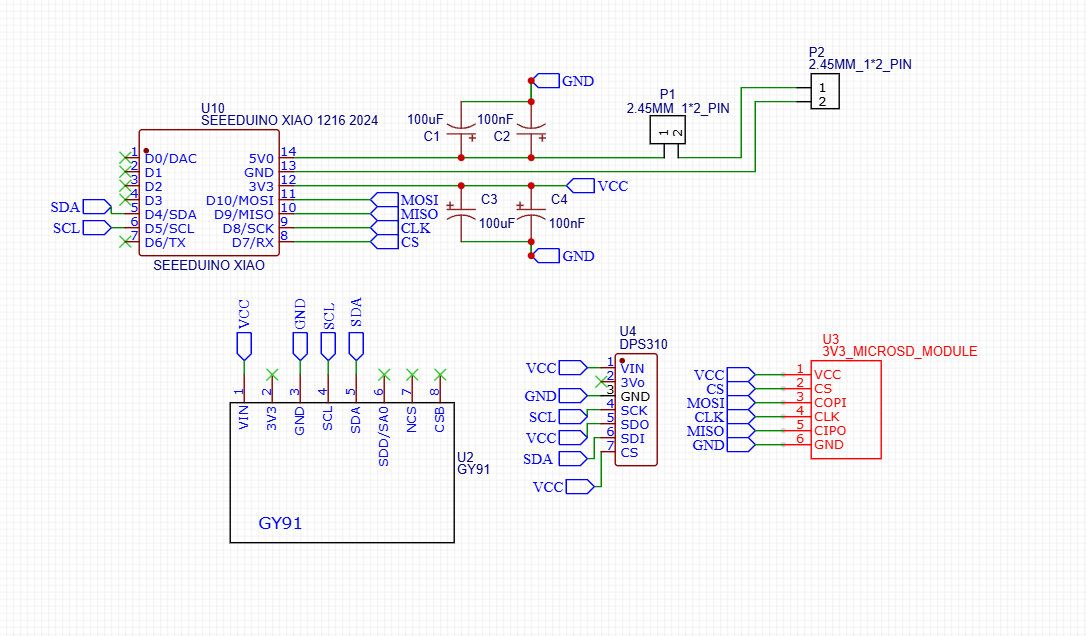
\includegraphics[width=0.8\linewidth]{esquematico_carga_util.png}
\caption{Diagrama esquemático de conexiones electrónicas de la carga útil.}
\label{fig:esquematico_payload}
\end{figure}

\subsection*{Montaje experimental}
El conexionado físico de los módulos y las pruebas preliminares de integración se realizaron inicialmente en placa de prototipado rápido para validar la integridad de las líneas de alimentación y bus I2C:

\begin{figure}[H]
\centering
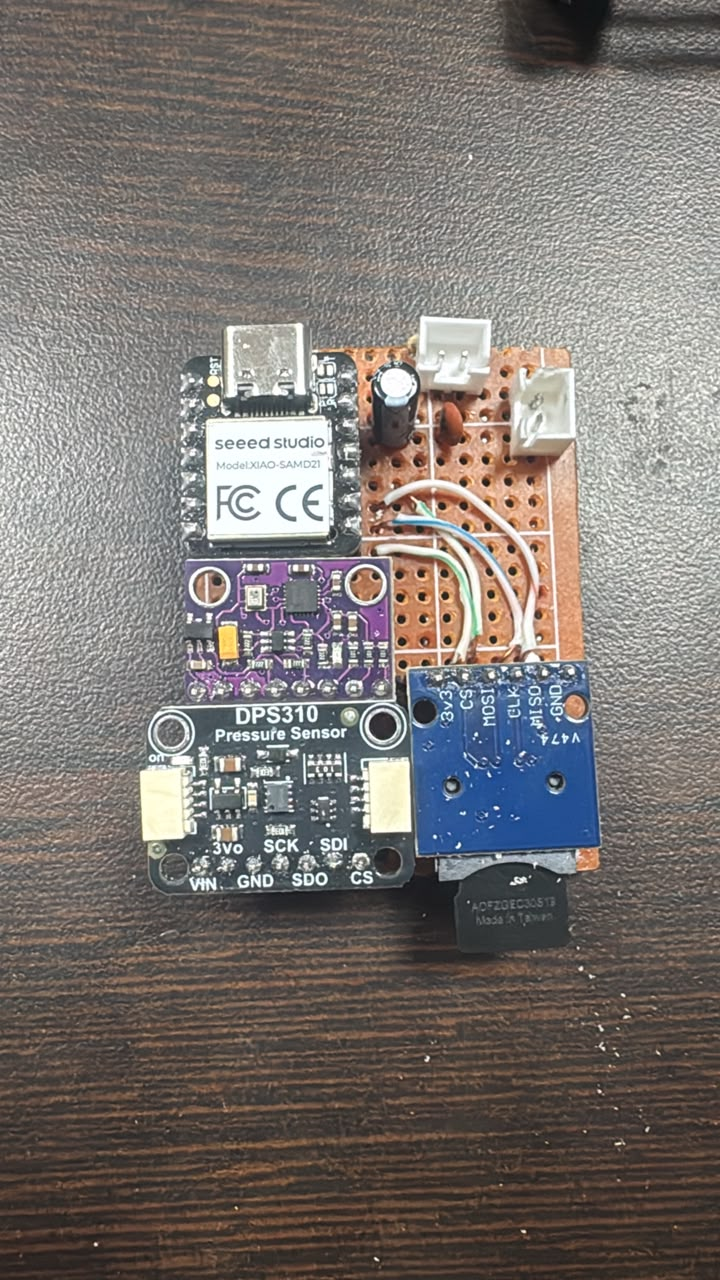
\includegraphics[width=0.75\linewidth]{montaje_experimental.jpg}
\caption{Montaje experimental físico y conexionado de la carga útil.}
\label{fig:montaje_payload}
\end{figure}

Para el vuelo final se desarrolló una placa de circuito impreso (PCB) fabricada mediante fresado CNC en placa de baquelita FR4, proporcionando alta rigidez y eliminando cables sueltos que pudieran desconectarse por choque dinámico:

\begin{figure}[H]
\centering
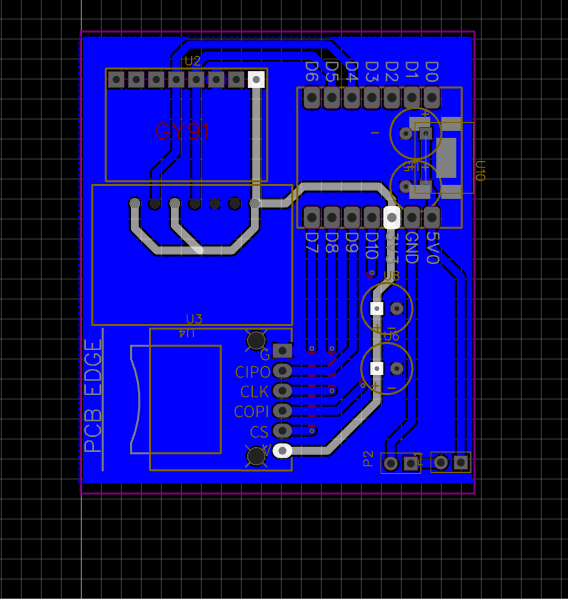
\includegraphics[width=0.75\linewidth]{pcb_carga_util.png}
\caption{Placa de circuito impreso (PCB) desarrollada para la carga útil.}
\label{fig:pcb_payload}
\end{figure}

\subsection*{Alimentación eléctrica}
El sistema se energiza mediante una batería recargable compacta de níquel-metal hidruro (NiMH) de \textbf{3,6 V y 150 mAh}, seleccionada por su estabilidad química ante variaciones de temperatura y nulo riesgo de inflamación frente a polímeros de litio. El consumo medio de corriente del conjunto (Seeeduino + sensores + micro-SD) es de aproximadamente 28 mA, garantizando una autonomía operativa superior a \textbf{3,5 horas}.

\subsection*{Respaldo de los datos principales}
Como salvaguarda ante una eventual falla mecánica o expulsión de la tarjeta microSD durante el shock de aterrizaje, las variables críticas del vuelo (altitud máxima en apogeo, velocidad máxima de ascenso, aceleración pico y tiempo total hasta el apogeo) se escriben directamente en la \textbf{memoria no volátil EEPROM} interna del microcontrolador al momento de detectarse el apogeo.

\subsection*{Telemetría y estación en tierra}
La carga útil de Categoría 2 opera bajo la modalidad de registro a bordo (\textit{data logger}), priorizando la confiabilidad y la ligereza del sistema. No obstante, para la lectura y análisis inmediato pos-vuelo en la zona de recuperación, se diseñó una interfaz gráfica desarrollada en Python (Tkinter/Matplotlib) que descarga los datos vía puerto serie USB y grafica instantáneamente la trayectoria:

\begin{figure}[H]
\centering
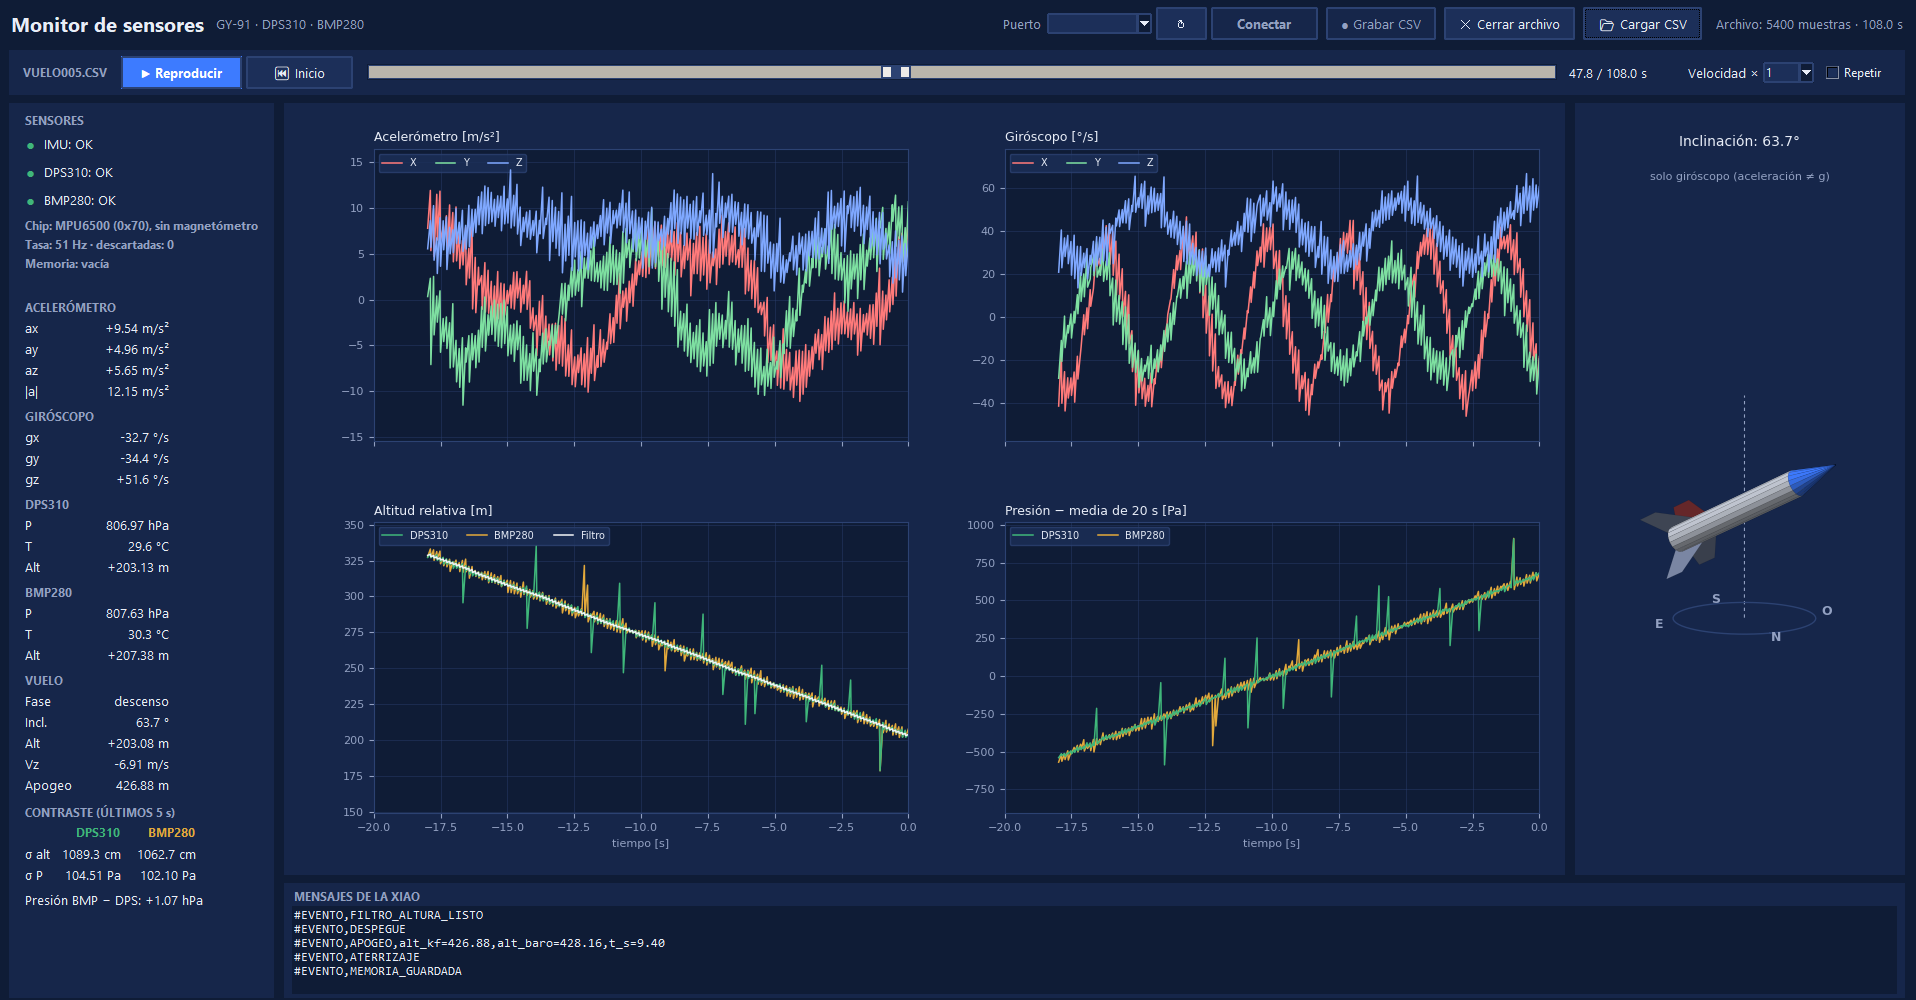
\includegraphics[width=0.85\linewidth]{interfaz_visualizacion.png}
\caption{Interfaz de usuario desarrollada para la visualización y análisis de datos pos-vuelo.}
\label{fig:interfaz_gui}
\end{figure}

\subsection*{Prueba de Banco en Tierra}
Para comprobar la estabilidad de los sensores y la fidelidad del filtro de Kalman antes del lanzamiento, se realizó una prueba de banco en tierra con una duración de 48 segundos simulando perturbaciones de movimiento:

\begin{figure}[H]
\centering
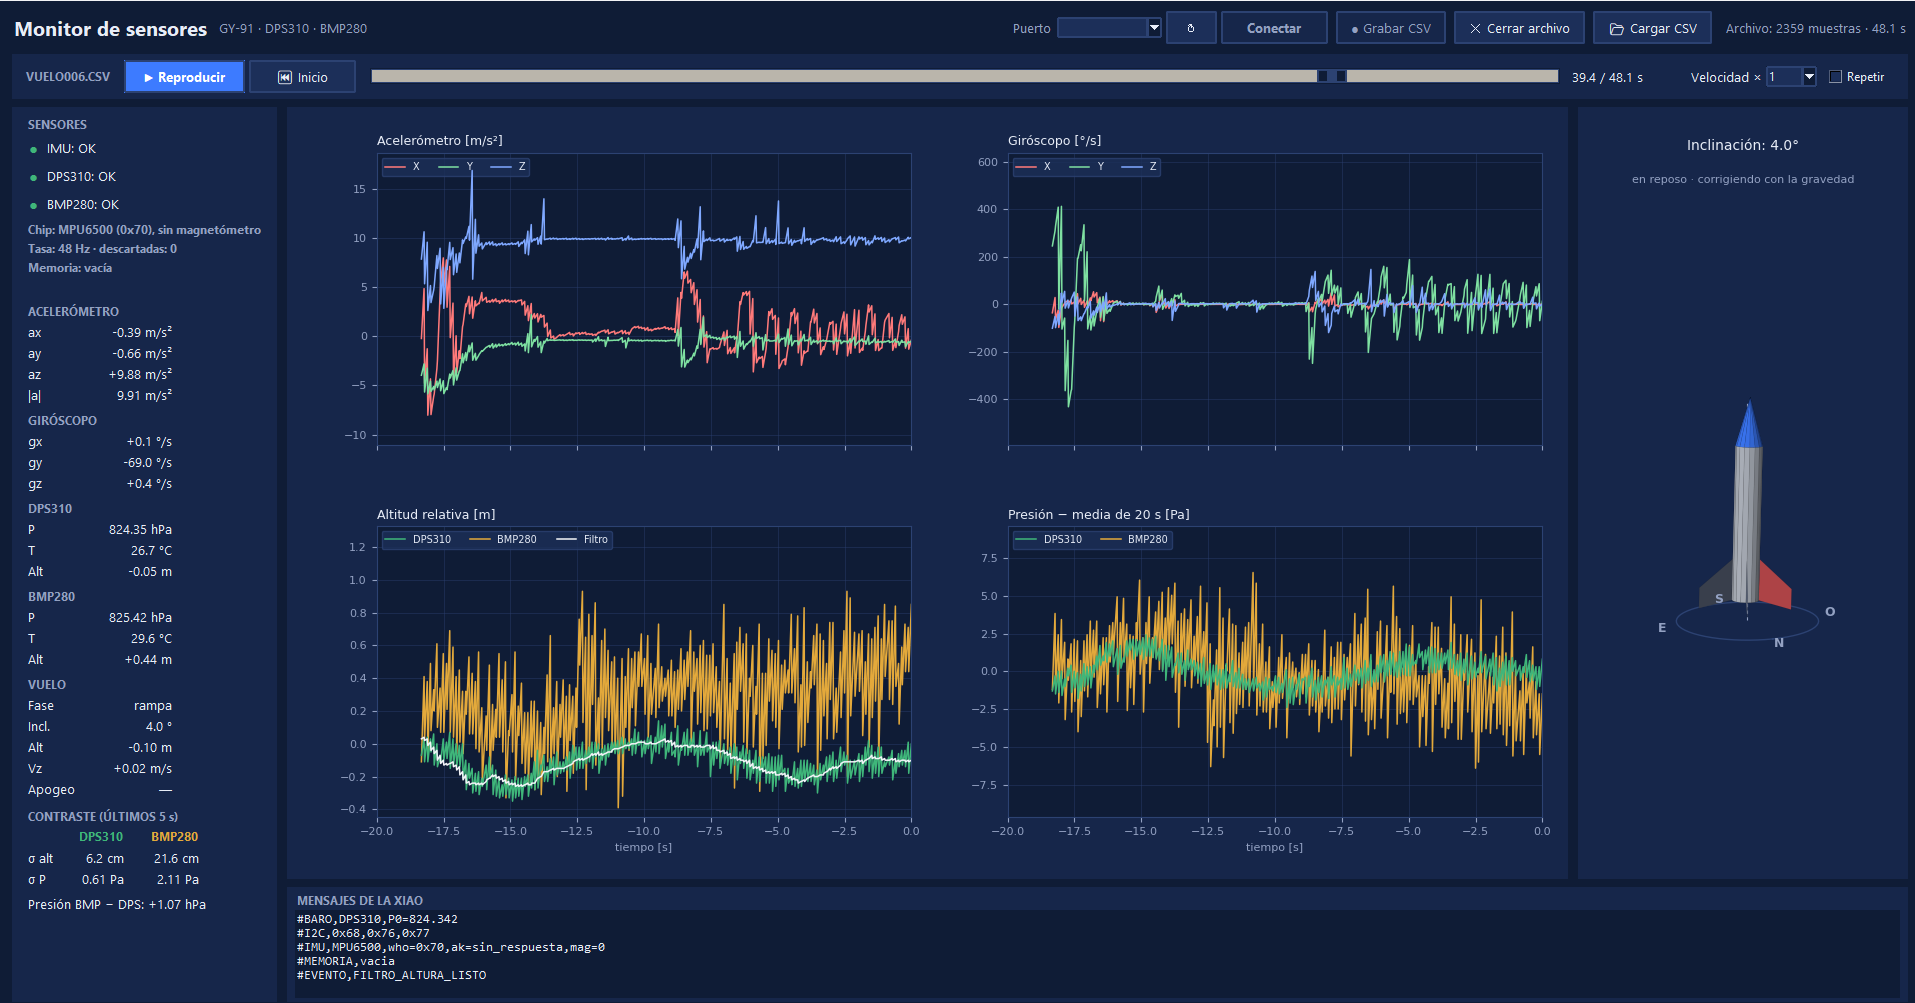
\includegraphics[width=0.85\linewidth]{prueba_banco_grafica.png}
\caption{Registro de la prueba de banco en tierra con sensor barométrico y filtro de Kalman.}
\label{fig:prueba_banco}
\end{figure}

La prueba demostró que el barómetro DPS310 posee una desviación estándar mínima ($< 0,08\text{ m}$) frente a sensores comunes y que el filtro de Kalman rechaza satisfactoriamente los picos de ruido sin presentar derivas artificiales de altitud.
